\documentclass[oneside, 11pt]{article}

\usepackage[T1]{fontenc}
\usepackage[utf8]{inputenc}
\usepackage[dutch]{babel}

\usepackage{fouriernc}
\usepackage[detect-all, load-configurations=binary,
            separate-uncertainty=true, per-mode=symbol,
            retain-explicit-plus, range-phrase={ tot }]{siunitx}

\usepackage{setspace}
\setstretch{1.2}

\setlength{\parskip}{\smallskipamount}
\setlength{\parindent}{0pt}

\usepackage{geometry}
\geometry{marginparwidth=0.5cm, verbose, a4paper, tmargin=3cm, bmargin=3cm, lmargin=2cm, rmargin=2cm}

\usepackage{float}

\usepackage[fleqn]{amsmath}
\numberwithin{equation}{section}
\numberwithin{figure}{section}

\usepackage{graphicx}
\graphicspath{{Figures/}}
\usepackage{subfig}

\usepackage{tikz}
\usetikzlibrary{plotmarks}

\usepackage{fancyhdr}
\pagestyle{fancy}
\fancyhf{}
\rhead{\thepage}
\renewcommand{\footrulewidth}{0pt}
\renewcommand{\headrulewidth}{0pt}

\usepackage{relsize}
\usepackage{xspace}
\usepackage{url}

\newcommand{\figref}[1]{Figuur~\ref{#1}}

\newcommand{\hisparc}{\textsmaller{HiSPARC}\xspace}
\newcommand{\kascade}{\textsmaller{KASCADE}\xspace}
\newcommand{\sapphire}{\textsmaller{SAPPHiRE}\xspace}
\newcommand{\jsparc}{\textsmaller{jSparc}\xspace}
\newcommand{\hdf}{\textsmaller{HDF5}\xspace}
\newcommand{\aires}{\textsmaller{AIRES}\xspace}
\newcommand{\csv}{\textsmaller{CSV}\xspace}
\newcommand{\python}{\textsmaller{PYTHON}\xspace}
\newcommand{\corsika}{\textsmaller{CORSIKA}\xspace}
\newcommand{\labview}{\textsmaller{LabVIEW}\xspace}
\newcommand{\daq}{\textsmaller{DAQ}\xspace}
\newcommand{\adc}{\textsmaller{ADC}\xspace}
\newcommand{\adcs}{\textsmaller{ADC}s\xspace}
\newcommand{\Adcs}{A\textsmaller{DC}s\xspace}
\newcommand{\hi}{\textsc{h i}\xspace}
\newcommand{\hii}{\textsc{h ii}\xspace}
\newcommand{\mip}{\textsmaller{MIP}\xspace}
\newcommand{\hisparcii}{\textsmaller{HiSPARC II}\xspace}
\newcommand{\hisparciii}{\textsmaller{HiSPARC III}\xspace}
\newcommand{\pmt}{\textsmaller{PMT}\xspace}
\newcommand{\pmts}{\textsmaller{PMT}s\xspace}

\DeclareSIUnit{\electronvolt}{\ensuremath{\mathrm{e\!\!\:V}}}

\DeclareSIUnit{\unitsigma}{\ensuremath{\sigma}}
\DeclareSIUnit{\mip}{\textsmaller{MIP}}
\DeclareSIUnit{\adc}{\textsmaller{ADC}}

\DeclareSIUnit{\gauss}{G}
\DeclareSIUnit{\parsec}{pc}
\DeclareSIUnit{\year}{yr}



\begin{document}

\title{Voorbeeldje}
\author{A. de Laat}
\date{}

\maketitle

\section{Begin}

In de natuur oefenen voorwerpen krachten op elkaar uit. Dit kan bijvoorbeeld
doordat twee voorwerpen met elkaar botsen. We kunnen hier denken aan
grote samengestelde voorwerpen voorwerpen, maar ook aan kleine voorwerpen.
Een scheikundige reactie is misschien wel te beschouwen als een soort
botsing van atomen (of moleculen) waardoor een (ander) molecule onstaat.

Botsingen zijn op twee manieren te beschouwen, elastische botsingen
en niet-elastische botsingen. Een scheikundige reactie is te beschouwen
als een niet-elastische botsing. Kernreacties zijn ook te beschouwen
als niet-elastische botsingen.


\section{Behoudswetten}

Bij botsingen bestuderen we systemen van verschillende objecten. We
kunnen bij\-voorbeeld denken aan een botsing van een scooterrijder met
een vuilnisbak. Dit is een scooterrijder/vuilnisbak systeem te noemen.
Volgens de derde wet van Newton
($\mathbf{F}_{actie}=-\mathbf{F}_{reactie}$) \footnote{Ik gebruik voor
de vector van de kracht "$\mathbf{F}$", de grootte wordt geschreven met
"$F$".} oefenen beide objecten in het systeem op ieder moment een even
grote maar tegengestelde kracht uit \footnote{Let op: Dit is een ander
situatie dan een object waarbij alle krachten die op dat object werken
in evenwicht zijn. Dit laatste is een bijzonder geval van de tweede wet
Newton.}. Voor en na de botsing is deze kracht 0N. Gedurende de botsing,
die voor beide objecten even lang duurt, zijn er twee even grote en
tegengestelde krachten. Als voorwerp I gedurende de botsing vertraagt,
versnelt voorwerp II. We kunnen deze (eenparig) versnelde bewegingen dus
nader bestuderen met de tweede wet van Newton:

\begin{equation}
    \mathbf{F}=m\mathbf{a}
\end{equation}

Meer tekst en na de botsing. Gedurende de botsing, die voor beide
objecten even lang duurt, zijn er twee even grote en tegengestelde
krachten. Als voorwerp I gedurende de botsing vertraagt, versnelt
voorwerp II. We kunnen deze (eenparig) versnelde bewegingen dus nader
bestuderen met de tweede wet van Newto.

\begin{figure}[H]
    \centering
    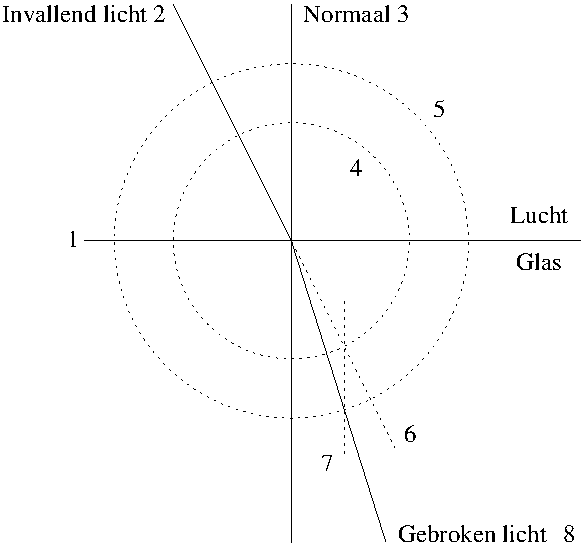
\includegraphics[scale=0.75]{vlak}
    \caption{De breking aan een plat vlak}\label{fig:vlak}
\end{figure}

Gedurende de botsing, die voor beide objecten even lang duurt, zijn er
twee even grote en tegengestelde krachten. Als voorwerp I gedurende de
botsing vertraagt, versnelt voorwerp II.

\begin{thebibliography}{9}
    \bibitem{tekst}
        Door N.G. Schultheiss, \emph{Botsen en Lenzen}, CC-BY-SA-3.0, via \hisparc
\end{thebibliography}

\end{document}
